\setchapterpreamble[u]{\margintoc}
\chapter{A Renewable Solution?}
\labch{renewable_solution}

In this chapter I will go over computing the amount of capacity to install, the amount of storage to install, the impact to expect on the grid, and the impact of a renewable mix versus what we will end up computing, a homogeneous system.

We have discussed this previously: we want a sustainable grid, looking at a first-order optimal solution at a horizon of 100 years. And in order to attain this goal, recall that we defined two main categories of scenarios.

\begin{itemize}
	\item 100\% Nuclear Scenario
	\item 100\% Renewable Scenario
\end{itemize}

The 100\% nuclear will first get rid of all the existing installed capacity, with the associated dismantling cost, and rebuild everything from scratch to cover the entirety of a country electricity needs. We will not consider exports or imports of electricity. The\sidenote[][-2mm]{Again, I cannot repeat that enough, we are after a first-order estimate} costs of this scenario will be computed over the next 100 years.

For the 100\% Renewable energy scenario, we will look at a solution consisting of a country relying entirely on solar, entirely on onshore wind or entirely on offshore wind production. All these scenarios will similarly get rid of the current nuclear fleet, and rebuild everything from scratch to a 100\% technology penetration.

Obviously, the one-technology scenario are a bit on the extreme side. The load factor considered in a renewable mix will be a little more advantageous due to a combined effect\sidenote[][-2mm]{You can have wind when you do not have solar, and vice versa. But keep in mind that the limiting factor will often be windless or low-wind nights, which are not uncommon}. We will estimate the impact of this second order effect later on. Finally, we will see what a renewable and nuclear mix could look like, and under what conditions it would make sense economically, societally, and physically.

Again, recall that we want only a simplistic first-order comparison. Our goal is not to build a complex model, optimized and tuned to decades of historical and projected data\sidenote[][-2mm]{Those models are set in an ideal Utopian world where crisis are non-existent and society is more stable than any other time in history. I am rooting for this, but I like to stay reasonable}. We aim to show what one can reasonably expect from various scenarios and draw conclusions from this. Policies have never been made on complex, perfectly optimized simulations. If the first order calculation does not agree with a complex model, it does not mean the complex model is wrong per se, but that its implementation is unlikely to work as intended, because humans are not always rational actors unfortunately.

Multiple scenarios will be tested from the two categories we defined.


\begin{kaobox}[frametitle=Scenarios to consider]

\begin{itemize}
	\item S1: Onshore Wind -- Pumped Hydro Storage
	\item S2: Onshore Wind -- Batteries
	\item S3: Offshore Wind -- Pumped Hydro Storage
	\item S4: Offshore Wind -- Batteries
	\item S5: Solar -- Pumped Hydro Storage
	\item S6: Solar -- Batteries
	\item S7: Nuclear
	\item S8\footnote{We can vary the share of each technologies. By default, we use 30\% onshore wind, 10\% offshore wind,  60\% solar mix, and 50\% batteries, 50\% pumped storage}: Renewable Mix -- Storage Mix
	\item S9\footnote{We can vary the share of each technologies. By default, we use 24\% wind onshore, 8\% wind offshore, 48\% solar, 20\% nuclear mix}: Nuclear -- Renewable Mix
\end{itemize}

Each of the scenarios will furthermore be tested for sensitivity by modifying parameters and looking at a range of future potentials, from pessimistic to optimistic depending on the energy source.

\end{kaobox}

\section{Recalling the Assumptions}

The question of electricity imports and global exchange is important, and a difficult one to account for. That is, if there is not enough electricity available in France, can I ask my neighbors to sell me some? In our first order calculation, we are considering that no, this is not an option. The reasoning why follows. Say you have a dark, cold, calm day in France. Your wind and solar energies sources are thus severely hampered. You technically would have three options.

\begin{itemize}
	\item Use your storage capacity
	\item Ask the neighbors
	\item Learn to not use electricity
\end{itemize}


Well, from multiple observations in Europe, when such a situation happens somewhere in France for example, things are not looking great in other parts of Europe, due to meteorological effects such as anticyclones and depressions. This is especially within immediate neighboring countries such as Germany or Spain. Any electricity the neighbors would produce would be used for their own needs, and put into their storage for future domestic use if any is left. Our main assumption is that the installed capacity is enough to power yourself, but that you are not building up out of the goodness of your heart for your neighbors\sidenote[][-2mm]{And I argue that it makes for a poor investment to try and overbuild your capacity even more to sell your surplus, as most of your surplus would happen when other countries are not especially in dire need}.

We also assume that consumption stays constant over time. Additionally, and importantly, the main assumption is that we want a world and a society that is not radically different from today, hence the ability to dispatch energy when and where you want it.

Another crucial point to consider is that the low-carbon grid we want needs to be sustainable\marginnote[-2mm]{You may come across articles or headlines that claim that the cost of transition to a fully decarbonized system is a given amount of trillions of dollars for a given country. This does not have to be false, but, again, we want a sustainable, long term grid. If we had a technology today that was able to completely decarbonize our grid for \$5 trillion dollars for a country like the USA and could be built in a month, it would be great, nay, incredible. But if I then told you that the lifetime of that technology is one year, so that every year, you needed to rebuild it anew, the cost would be incredibly high and crippling to the current world economy. Even if this was doable, it would then go against the assumption that we do not want to change to a radically different society in a very short time span. In my experience, this is ignored most of the time, and is coherent with the easy pitfalls of "this is the next-generation problems" tropes}. It is not enough to switch to a low carbon system and, once its lifetime is up, give up on it. Lifetime cycles need to be accounted for over a long period. In this demonstration, we consider 100 years to be a representative period. We will drop this to 50 years to see the sensitivity.


\begin{table}[ht]
\caption[Input Data and Notations]{Input Data and Notations}
\labtab{input_notations}
\begin{tabular}{ c c c }
	\toprule
	Data & Notation & Units\\
	\midrule
	Annual Energy Production Needs & $E_a$ & TWh \\
	Installed Capacity & $P_i$ & GW\\
	Technology Load Factor & $f$ & \% \\
	Peak Production & $p_{max}$ & \% \\
	Energy Storage Capacity & $E_s$ & TWh\\
	Power Storage Capacity & $P_s$ & GW \\
	Power Excess & $P_e$ & GW \\
	Storage Round-Trip Efficiency & $e$ & \% \\
	Installed Capacity with Storage & $P_{i,s}$ & GW \\
	Minimum Yearly Need & $P_{min}$ & GW \\
	Energy Storage Fraction & $f_s$ & \% \\
	Installation Costs & $C_i$ & \$ \\
	Storage Costs & $C_s$ & \$ \\
	Dismantling Costs & $C_d$ & \$ \\
	Grid Costs & $C_g$ & \$ \\
	Duration of Storage need & $t$ & hours \\
	\bottomrule
\end{tabular}
\end{table}


\section{How Many GigaWatts?}

We have seen from \vrefch{transition_needs} the amount of energy to be produced annually, in TWh, per country of interest. In that chapter we also derived the load factor per technology, in the latest years.


An important factor to consider now is the capacity of electricity you need to install in order to obtain this necessary energy produced at the end of any given year. This is shown in equation~\ref{eqn_power_installed}.

\begin{remark}
In order to obtain the energy generated over a year in Wh, one needs to multiply the power installed by the number of hours in a year\sidenote[][-2mm]{Mind the units! Recall that $E_a$ is in Terrawatt-hour, which is a thousand Gigawatt-hour and a billion kilowatt-hour. So, the $P_i$ obtained will be in Terrawatt. We are most used to dealing with installed capacity in Gigawatt, which implies a multiplication by $10^{-3}$ of your result}.

\begin{equation}\label{eqn_power_installed}
P_i = \frac{E_a}{f * 8760}
\end{equation}

\end{remark}

\section{Storage Requirements}

As discussed, energy storage is a fundamental piece of any 100\% renewable scenario. So, exactly how much storage do we need?

To answer this question, the first thing we need to know is:

\begin{itemize}
\item What is the maximum period of time where our needs could be unmet?
\end{itemize}

An important thing to note here is that when we say that the needs are not meet, it does not mean that we get no power from our installed capacity. It means that we do not get enough power from our installed capacity. 10 days of wind production at 20\% is equivalent to 2 days of no wind at all.

Common scenarios are a gloomy week, or a sustained storm. In those cases, solar and wind production will be hampered. It is not unreasonable, to think that 7 days of storage would be needed. Keep in mind that if you do not have enough storage in place and run out, the whole economy stops. We will modify the duration to test the sensitivity, from 1 to 7 days.


\begin{remark}
The energy to store is given by~\ref{energy_store}, $t$ varying between 1 and 7 days (it has to be given in number of hours).

\begin{equation}\label{energy_store}
E_s = t * \frac{E_a}{8760}
\end{equation}

\end{remark}

Round-trip efficiency represent the fraction of the electricity that you put in that you can expect to get back. Indeed, you will not get back everything you sent to your storage, due to cable losses, inverter or mechanical losses, and various other factors. This efficiency is variable between technologies and over time. A good approximation is between 65\% and 85\%\sidenote[][-2mm]{As an example, for pumped storage, the main sources of losses are approximately 5\% to the network itself, 80\% to the pumping stations and 85\% to the turbines, which translates to 65\%, and thus a loss to storage of 35\%.}. 

This has a strong implications. In order to get back the energy you would need, you have to send $\frac{1}{0.85} = 1.18$ to $\frac{1}{0.65} = 1.55$ times as much electricity. This has a potential impact on the capacity that has to be installed to begin with.

We will assume that this does not matter for our first order calculation, and that we have enough power generation to fill in sufficient storage power capacity by default. Additionally, we consider that the extra power generated when demand is low can be easily curtailed or used in alternate, non-time sensitive process. This encompasses hydrogen production or desalination, for example, two energy intensive processes\sidenote[][-2mm]{Energy is only one of the drivers of these processes difficulties.}.



\begin{kaobox}[frametitle=What we have said]
Wind and Solar can be down or low for extended periods of time, during which batteries have to pick up the slack. This represents $x$ TWh over the year and gives us a battery output required assuming a duration period to cover of $y$ days.

While this may seem to not take advantage of a combining effect, this is actually a reasonable assumption in the real, non-perfectly-optimized, world. In such optimized modeling simulations, real world constraints such as geopolitics and social difficulties are often ignored or misrepresented.

\end{kaobox}


\section{Renewable Mix Impact}

We have seen an approximation, which we will use for our simplified scenarios S1 through S6\todo{Improve this part. We can maybe remove the production hours graphs and simply assume that we need to meet consumption assumption an X day period to compensate for. We need to show how a mix impacts the storage needs by combining hourly data from both wind and solar over a period. The question is thus to find hourly data for solar production in a given year and combine it with hourly data for wind production in the same year and same location, to compute the storage requirements}. Let's see how we can factor in a more realistic system, where a mix of renewable energies is used, with wind, solar and hydro working in unison over larger areas.

To answer this question, the first thing we need to know is:

\begin{itemize}
\item Given a mix of renewable energies, what is the maximum period of time where our needs are not met?
\end{itemize}

This will vary depending on the mix you define.


\begin{figure}[ht]
	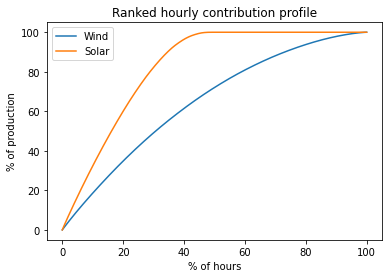
\includegraphics[width=1.0\textwidth]{renewable_production_hours_ranked}
	\caption[Percent of hours in a year contributing to a percent of the output, ranked by importance]{Percent of hours in a year contributing to a percent of the output, ranked by importance.}
	\labfig{renewable_production_hours_ranked}
\end{figure}

The \vreffig{renewable_production_hours_ranked} may be a bit difficult to read, so let me spend some time explaining what went on here. In order to generate this plot, I used one year of hourly power output for both wind and solar power. The solar data was simulated over Texas using synthetic solar photovoltaic from NREL. The wind data was downloaded from the ERCOT website, the Texan grid operator. This data consequently approximates potential redistribution of power generation between different part of the state of Texas.

Knowing the power generated every hour of the year, I then ranked them from most productive to least productive. So, if you take the solar data for example, the "noons" of the year are first, and the nightly hours come later, not contributing any power to the production. From that, I then plotted where each hour falls in the year ranking against the percentage of production.

In other words, what this graph shows is that for solar power, once you reach the 40\% of the top contributing hours, you have generated all the yearly power. The remaining 60\% do not contribute power. This is logical, as it is night 50\% of the time and your panels are more efficient in direct sunlight than in the evening, when it gets hit only by diffuse sunlight.

Another way of interpreting this graph is that 80\% of solar power production is done in only 30\% of the time during the year, leaving you at risk of not meeting production demand the rest of the time because you can easily find period where multiple consecutive hours are in those 70\% remaining hours.

Wind is less predictable, but has more contributing hours during a year. You do not have a clear cycle like nights and days, and it varies a bit more regionally than the sun irradiance. 80\% of the production from wind power comes from 60\% of the time, leaving you at risk during 40\%. Using this data, what we can conclude as a first order approximation is that your needs, with solar, would be covered 30\% of the time, while they would be covered 60\% of the time for wind\sidenote[][-2mm]{A complex model can give better results there, by combining the solar or wind data with an estimation of the hourly load notably, at the risk of over-optimization leading to a less resilient grid and more frequent blackouts. Our approach is still a pretty good first order approximation of the scale we are talking about.}.

Consequently, we can say that in the most favorable situation, wind would cover for solar at night, and wind is low only during the day.

\begin{remark}
In that case, based on a reasonable 80\% of the total production viability:

\begin{itemize}
\item It's sunny enough for 30\% of the time, and not windy enough for 40\% of the time
\item It's windy enough for 60\% of the time, and not sunny enough for 70\% of the time
\end{itemize}

So, on first approximation, we can say that 10\% of the energy need cannot be met, even under the most ideal, fairy tale scenario.

\end{remark}

One can consider adding hydroelectricity or geothermal to the mix and think that this could meet 100\% of the demands and to not have a storage requirements\sidecite{hoste2009matching,brown2018synergies}. It has however been shown to be reliant on assumptions that are on the very optimistic side\sidecite{boretti2020cost,clack2017evaluation}. A different way to look at it is that it may work for tight regions with strong interconnections and links, such as the European Union and the United States of America, and in a beautifully engineered infrastructure. Besides that, it is a lot more difficult to imagine such level of cooperation, especially concerning such a vital infrastructure\sidenote[][*6]{From a purely geopolitical and national security perspective, it is not far-fetched to consider the impact on balance of power at small and abrupt time scale.}.

In this section, we will consider the short term unpredictable variability of solar and wind, and consider that even only 10\% of the energy needs have to come from storage\sidenote[][*6]{Keep in mind that while this is theoretically possible, it is physically unlikely to be the case. That's the limitation with theoretical models, they tend to assume that everything works a bit too much as expected}.


\begin{remark}

In this renewable energy mix scenario, which does imply an important paradigm shift in society consumption and grid operation, the amount of storage needed consequently is given by~\ref{energy_store}, $t$ varying between 1 and 7 days (it has to be given in number of hours) and becomes:

\begin{equation}\label{energy_store}
E_s = f_s * t * \frac{E_a}{8760}
\end{equation}

Here, we assume that an optimist assumption for the fraction of energy to store is $f_s = 10\%$.

Note that we still consider periods up to 7 days because of the inherent uncertainty of the system.

\end{remark}




\section{Grid impact}

We are making the assumption here that the grid is able to deal with a lot of excess energy, or that this is used for non-time-dependent processes like hydrogen production, desalination, or other. This comes with grid requirements which can be very difficult to meet.

Grids have been designed to accommodate for around the power capacity that is currently installed, in a mostly centralized, optimized, system. In order to move to a 100\% renewable system, hence mostly decentralized, non-optimized, system, grid developments will be necessary, and transmission lines will have to be built. In terms of cost, it is no secret that it is a lot more expensive to install 500 lines of 100 MW (accommodating an installed capacity of 50 GW) than 25 lines of 2 GW (accommodating the same installed capacity). Materials, public works, distance covered, all those and more factor into the increased price.

More importantly, the installed capacity being greater, the grid has to be reinforced to account for the maximum expected output. While the load factor over the year is relatively low for wind or solar, you will have peaks throughout the year at up to 70\% and 90\% of the installed capacity respectively\sidenote[][-2mm]{A sunny day at noon, a windy day on all your wind farms, and all of the sudden you have way more energy than you know what to do with!}. 

You are presented with three basic options for this energy.
\begin{itemize}
\item Store it
\item Use it
\item Dump it
\end{itemize}

The first option is to store it for future use as long as you have the installed storage power capacity. Given your requirements, this has to be done in priority. The second option is to use that excess energy for auxiliary uses, such as hydrogen production. This is not as simple as it seems, and is unfortunately not a magical solution, though it has a lot of merits. The third option is to accept the loss and curtail your production.


\begin{remark}
Consequently, the grid should be ready to deal with an excess power up to what is given in the following equation.

\begin{equation}\label{excess_power}
P_e = P_i * p_{max} - P_{min}
\end{equation}
\end{remark}


\section{Energy Mix}

As mentioned several times, we are considering homogeneous scenarios. The production comes either from solar, or from wind, or from nuclear, and so forth. In reality, a mix would be beneficial for multiple reasons, including economical competition and load factor smoothing. Load factor smoothing would be the idea that you have nights, you have windless days, but since you have windy nights or sunny calm days, by definition the overlaps increases the load factor of your system.

We can use the simulated data discussed previously to quickly estimate the impact.

\begin{itemize}
\item Get the solar production per hour
\item Get the wind production per hour
\item Sum the two
\item Get the load factor for solar only
\item Get the load factor for wind only
\item Get the load factor for combination
\end{itemize}



\section{The Digest}


\begin{kaoboxgreen}[frametitle=Main Takeaways]

\begin{itemize}
\item We derive the main simple equation to be used to approximate the costs of a scenario
\item The capacity to install per scenario is given depending on a constant need assumption
\item The storage consequence is approached, and we go easy on it
\end{itemize}
  
\end{kaoboxgreen}